\documentclass[class=report, crop=false, 12pt,a4paper]{standalone}
\usepackage{enumitem}
\usepackage{tikz}
\usetikzlibrary{shapes.geometric, arrows}
\usepackage{float}
\usepackage{graphicx}
\usepackage{multicol}
\usepackage{siunitx}
\usepackage{mathtools}
\usepackage{amsmath}
\usepackage{amssymb}
\usepackage{commath}
\usepackage[normalem]{ulem}
\usepackage[a4paper,width=150mm,top=25mm,bottom=25mm]{geometry}
\begin{document}
\subsection*{Stages in a measurement system}
\begin{figure}[H]
  \centering
  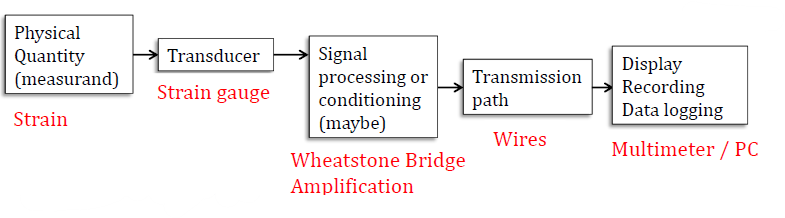
\includegraphics[width = 0.8 \textwidth]{../img/diagram38.png}
\end{figure}
\section{Amplifiers}
\begin{figure}[H]
  \centering
  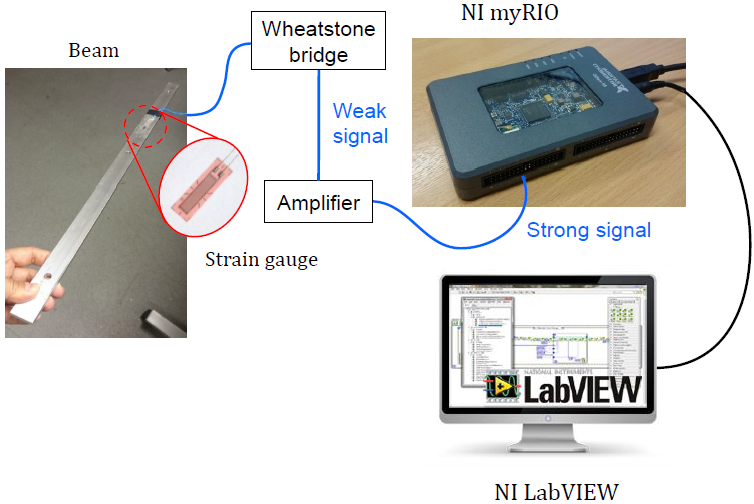
\includegraphics[width = 0.7\textwidth]{../img/diagram39.png}
\end{figure}
The voltage output from a transducer tends to be weak and this needs to be amplified. Operational amplifiers are normally around 1\si{\centi\meter} in size.
\begin{figure}[H]
  \centering
  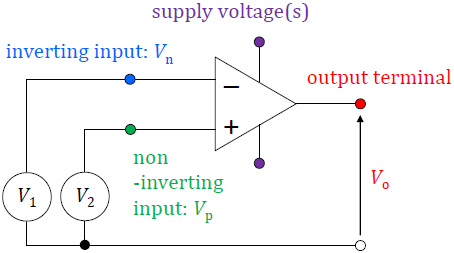
\includegraphics[width = 0.7\textwidth]{../img/diagram40.png}
\end{figure}
\begin{equation}
  V_0 = A_v (V_p - V_n) = A_v (V_2 - V_1)
\end{equation}
Where $A_v$ is the gain and $(V_p - V_n)$ can be from a Wheatstone bridge. Operational amplifiers are quite an old technology (since WW2) and are still used because they are cheap and convenient.
\begin{figure}[H]
  \centering
  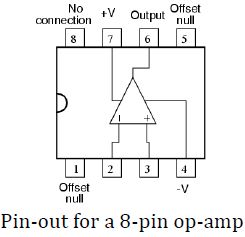
\includegraphics[width = 0.5\textwidth]{../img/diagram41.png}
\end{figure}
\begin{figure}[H]
  \centering
  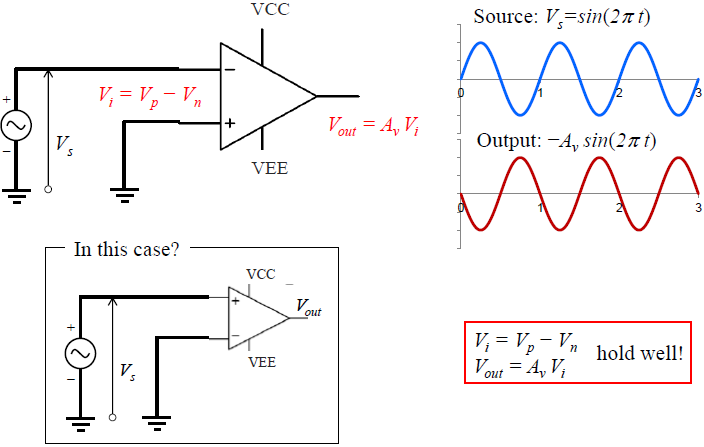
\includegraphics[width = 0.7\textwidth]{../img/diagram42.png}
\end{figure}
\subsection{Equivalent op-amp circuit and conditions of an ideal op-amp}
\begin{figure}[H]
  \centering
  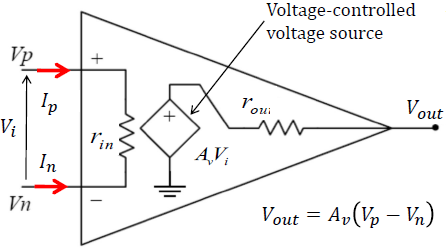
\includegraphics[width = 0.7\textwidth]{../img/diagram43.png}
\end{figure}
Terminology:
\begin{itemize}
  \item Differential input voltage: $V_i = V_p - V_n$
  \item Input resistance: $r_{in}$
  \item Output resistance: $r_{out}$
  \item Open-circuit output voltage: $V_{out}$
  \item Differential voltage gain: $A_v$
\end{itemize}
\begin{center}
  \begin{tabular}{ |c|c| } 
    \hline
    Conditions of an ideal op-amp & In reality \\
    \hline
    \hline
    No current into input terminals: $I_p = I_n = 0$ & \\
    \hline
    Infinite input resistance: $r_{in} \rightarrow \infty$ & $r_{in} > 200 \si{\kilo \ohm}$\\
    \hline
    Zero Output resistance $r_{out} = 0$ & $r_{out} < 1 \si{\kilo\ohm}$\\
    \hline
    Infinite differential (or open-loop) gain $A_v \rightarrow \infty$ & $A_v > 100,000$\\
    \hline
    Zero common-mode voltage gain $A_{cm} = 0$ & $A_v$ also frequency dependant\\
    \hline
  \end{tabular}
  \end{center}
\end{document}